\section{Исследовательский раздел}
В данном разделе производится вычислительные эксперименты.
\subsection{Системные характеристики}
Характеристики виртуальной машины на котором производится эксперимент:

\begin{itemize}
    \item Операционная система: Ubuntu 22.04 LST;
    \item Версия ядра: Linux version 6.5.0-15-generic;
    \item Объем оперативной памяти: 10ГБ;
\end{itemize}

\subsection{Результаты выполнения работы}

Запустить Makefile

\captionsetup{justification=centering,singlelinecheck=off}
\begin{figure}[h!]
	\centering
		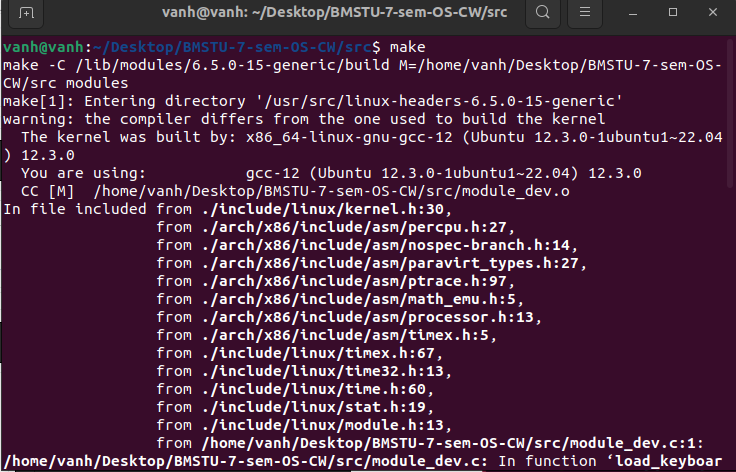
\includegraphics[,scale=0.6]{./img/3.png}
		\label{img:3}
\end{figure}

\captionsetup{justification=centering,singlelinecheck=off}
\begin{figure}[h!]
	\centering
		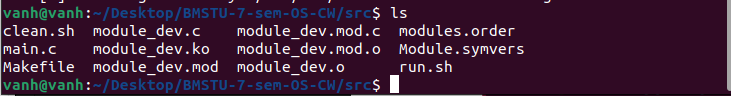
\includegraphics[,scale=0.6]{./img/4.png}
		\label{img:4}
\end{figure}
\break

Виртуальный файл создан

\captionsetup{justification=centering,singlelinecheck=off}
\begin{figure}[h!]
	\centering
		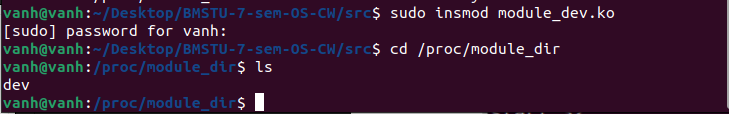
\includegraphics[,scale=0.6]{./img/5.png}
		\label{img:5}
\end{figure}

Пользовательская программа обнаруживает события подключения и отключения гарнитуры.

\captionsetup{justification=centering,singlelinecheck=off}
\begin{figure}[h!]
	\centering
		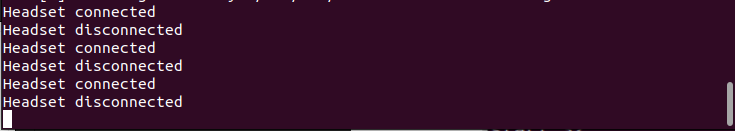
\includegraphics[,scale=0.6]{./img/6.png}
		\label{img:6}
\end{figure}

\captionsetup{justification=centering,singlelinecheck=off}
\begin{figure}[h!]
	\centering
		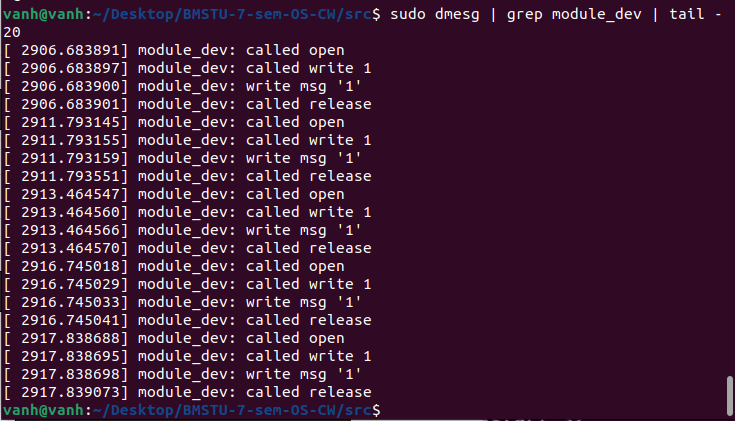
\includegraphics[,scale=0.6]{./img/7.png}
		\label{img:7}
\end{figure}